\chapter[Sprint 5 : Aide à la décision et finalisation]{Sprint 5 : Aide à la décision, rapports pondérés\\et finalisation de la plateforme}
\begin{spacing}{1.2}
\minitoc
\thispagestyle{MyStyle}
\end{spacing}
\clearpage

\providecommand{\screenshot}[2]{%
  \IfFileExists{../screenshoot/#1}{%
    \includegraphics[width=0.9\textwidth,height=12cm,keepaspectratio]{../screenshoot/#1}%
  }{%
    \fbox{\parbox[c][4.5cm][c]{0.9\textwidth}{\centering\itshape
      Capture d'écran à insérer~: #2\\[4pt]
      \normalfont\small(fichier attendu~: \texttt{screenshoot/#1})}}%
  }%
}

\section{Introduction}

Le cinquième et dernier sprint enrichit la plateforme de ses fonctionnalités d'aide à la décision et la prépare au déploiement. Il introduit l'analyse multimodale post-entretien, la comparaison et le classement des candidats, le tableau de bord administrateur, puis consolide la sécurité et la conformité avant la phase de finalisation, de tests et de durcissement.

\section{Objectifs du sprint}

L'objectif principal de ce sprint est défini comme suit~:

\begin{quote}
\itshape Compléter NextHire par ses fonctionnalités d'aide à la décision, rapport d'entretien pondéré, analyse multimodale et comparaison des candidats, et finaliser la plateforme (tableau de bord administrateur, sécurité, conformité RGPD, tests et déploiement), la décision finale demeurant celle du recruteur.
\end{quote}

\subsection{Backlog du sprint}

Le tableau~\ref{tab:backlog-s5} présente le backlog du Sprint~5.

\begin{table}[H]
  \centering
  \footnotesize
  \renewcommand{\arraystretch}{1.3}
  \setlength{\tabcolsep}{5pt}
  \begin{tabularx}{\textwidth}{|>{\centering\arraybackslash}p{1.1cm}|>{\raggedright\arraybackslash}X|>{\centering\arraybackslash}p{1.8cm}|}
    \hline
    \rowcolor{blue!10}
    \textbf{ID} & \textbf{Récit utilisateur} & \textbf{Priorité} \\
    \hline
    S1 & En tant que recruteur, je veux un rapport d'entretien pondéré selon les critères du poste. & Haute \\
    \hline
    S2 & En tant que recruteur, je veux comparer et classer les candidats d'un même poste. & Haute \\
    \hline
    S3 & En tant que recruteur, je veux revoir en détail un entretien terminé (transcription, scores, intégrité). & Haute \\
    \hline
    S4 & En tant qu'administrateur, je veux superviser l'activité de la plateforme via un tableau de bord. & Moyenne \\
    \hline
    S5 & En tant qu'utilisateur, je veux que mes données soient protégées (RBAC, RGPD, chiffrement). & Haute \\
    \hline
  \end{tabularx}
  \caption{Backlog du Sprint~5 : Aide à la décision et finalisation.}
  \label{tab:backlog-s5}
\end{table}

\section{Concept de l'aide à la décision}

À l'issue des entretiens, NextHire assiste le recruteur dans sa décision sans jamais s'y substituer. Cette aide repose sur trois apports complémentaires~: un \textbf{rapport d'entretien pondéré}, produit par l'agent selon les critères du poste (compétences techniques, communication, expérience, comportement, intégrité)~; une \textbf{analyse multimodale} post-entretien, qui ajoute des indices affectifs (émotion faciale, sentiment vocal) à titre contextuel~; et un \textbf{classement multicritères} des candidats pour un même poste.

Conformément au principe de décision humaine retenu dès la conception, ces éléments \textit{informent} le recruteur~: aucune embauche n'est décidée automatiquement, et la décision finale reste une action explicite et tracée.

\section{Conception détaillée et architecture}

\subsection{Génération du rapport post-entretien}

La figure~\ref{fig:seq-report} illustre le flux de génération du rapport post-entretien,
déclenché automatiquement dès la fin de la session. Le rapport final combine l'évaluation
pondérée de l'agent IA, dont les poids sont configurés par offre via le Job Wizard et
somment à 100 (par exemple~: technique 40\,\%, communication 20\,\%, expérience 20\,\%,
comportement 10\,\%, intégrité 10\,\%), et l'analyse multimodale produite par le service
Analysis via un pipeline LangGraph.

\begin{sloppypar}
\begin{enumerate}
  \item \textbf{Déclenchement.} Dès que l'agent retourne \texttt{done:true}, le backend
        récupère le snapshot de la session (transcription, évaluations IRT, critères du
        poste) depuis MongoDB pour construire l'évaluation pondérée.

  \item \textbf{Analyse post-entretien.} Le backend déclenche le service Analysis en
        arrière-plan (fire-and-forget). Ce service exécute un pipeline LangGraph : il
        récupère le document complet de la session, appelle un LLM (fournisseur configurable~:
        Gemini, NVIDIA NIM, OpenAI, Anthropic ou Ollama local) pour analyser
        la transcription, évaluer les compétences et produire des recommandations, puis
        persiste la timeline comportementale dans MongoDB.

  \item \textbf{Construction du rapport recruteur.} Le backend assemble le rapport final
        à partir du snapshot de l'agent, du rapport d'intégrité et des résultats de
        l'analyse, le persiste dans MongoDB et notifie le client de la fin de la session.

  \item \textbf{Consultation.} Le recruteur ouvre la fiche depuis le tableau de bord. Le
        backend renvoie le rapport complet (scores, violations, transcription,
        recommandations de l'IA).
\end{enumerate}
\end{sloppypar}

\begin{figure}[H]
  \centering
  \resizebox{\textwidth}{!}{%
  \begin{tikzpicture}[
    font=\scriptsize,
    >={Stealth[length=2mm]},
    msg/.style={->, thin},
    ret/.style={->, thin, dashed},
    lbl/.style={font=\tiny, fill=white, inner sep=1pt, midway, above},
    lifeline/.style={dashed, thin, gray!70},
    phdr/.style={draw, fill=blue!12, rounded corners=2pt, align=center,
                 font=\scriptsize\bfseries, minimum height=0.65cm, minimum width=2.7cm},
  ]

  %% ── Participants ──────────────────────────────────────────────────────
  \node[phdr] at ( 0,  0) {React\\(Recruteur)};
  \node[phdr] at ( 4.5,0) {Node.js\\(:3001)};
  \node[phdr] at (10,  0) {Analysis Service\\(:8090)};
  \node[phdr] at (15.5,0) {LLM Provider\\(Gemini / NVIDIA / ...)};
  \node[phdr] at (21,  0) {MongoDB};

  %% ── Lifelines ─────────────────────────────────────────────────────────
  \draw[lifeline] ( 0,  -0.38) -- ( 0,  -14.5);
  \draw[lifeline] ( 4.5,-0.38) -- ( 4.5,-14.5);
  \draw[lifeline] (10,  -0.38) -- (10,  -14.5);
  \draw[lifeline] (15.5,-0.38) -- (15.5,-14.5);
  \draw[lifeline] (21,  -0.38) -- (21,  -14.5);

  %% ════════════════════════════════════════════════════════════════════════
  %% 1. Déclenchement
  %% ════════════════════════════════════════════════════════════════════════
  \node[font=\tiny\bfseries, anchor=east] at (-0.3,-0.75) {1.};
  \draw[->] (4.5,-0.75) -- ++(0.6,0) -- ++(0,-0.40) -- ++(-0.6,0);
  \node[font=\tiny, anchor=west] at (5.15,-0.95)
    {buildWeightedEvaluation(agentSnapshot, criteria)};
  \draw[msg] (4.5,-1.60) -- node[lbl] {findOne(callRoom) : transcript + integrityEvents} (21,-1.60);
  \draw[ret] (21,-2.20) -- node[lbl] {\{transcription, evaluations, violations\}} (4.5,-2.20);

  %% ════════════════════════════════════════════════════════════════════════
  %% 2. Analyse post-entretien
  %% ════════════════════════════════════════════════════════════════════════
  \node[font=\tiny\bfseries, anchor=east] at (-0.3,-2.85) {2.};
  \draw[msg] (4.5,-2.85) -- node[lbl] {POST /api/interviews/\{id\}/analyze-video} (10,-2.85);
  \draw[msg] (10,  -3.50) -- node[lbl] {findOne(callRoom) \{full document\}} (21,-3.50);
  \draw[ret] (21,  -4.10) -- node[lbl] {\{transcription, visionEvents, agentEvaluations\}} (10,-4.10);
  %% self-arrow: LangGraph pipeline
  \draw[->] (10,-4.70) -- ++(0.6,0) -- ++(0,-0.40) -- ++(-0.6,0);
  \node[font=\tiny, anchor=west] at (10.70,-4.90) {LangGraph pipeline (analyse multimodale)};
  \draw[msg] (10,  -5.60) -- node[lbl] {chat.completions(transcript + job\_context + criteria)} (15.5,-5.60);
  \draw[ret] (15.5,-6.20) -- node[lbl] {\{skills\_scores, strengths, gaps, recommendations\}} (10,-6.20);
  \draw[msg] (10,  -6.85) -- node[lbl] {PATCH callRoom \{behavioralTimeline, analyzed: true\}} (21,-6.85);
  \draw[ret] (10,  -7.45) -- node[lbl] {\{status: done\}} (4.5,-7.45);

  %% ════════════════════════════════════════════════════════════════════════
  %% 3. Construction du rapport recruteur
  %% ════════════════════════════════════════════════════════════════════════
  \node[font=\tiny\bfseries, anchor=east] at (-0.3,-8.10) {3.};
  \draw[->] (4.5,-8.10) -- ++(0.6,0) -- ++(0,-0.40) -- ++(-0.6,0);
  \node[font=\tiny, anchor=west] at (5.15,-8.30)
    {buildRecruiterReport(snapshot, integrity, analysis)};
  \draw[msg] (4.5,-9.00) -- node[lbl] {PATCH callRoom \{status:ended, recruiterReport, integrityReport\}} (21,-9.00);
  \draw[ret] (21, -9.60) -- node[lbl] {200 OK} (4.5,-9.60);
  \draw[ret] (4.5,-10.15) -- node[lbl] {emit("interview-ended", \{overallScore, reportReady: true\})} (0,-10.15);

  %% ════════════════════════════════════════════════════════════════════════
  %% 4. Consultation du rapport (recruteur)
  %% ════════════════════════════════════════════════════════════════════════
  \node[font=\tiny\bfseries, anchor=east] at (-0.3,-10.90) {4.};
  \draw[msg] ( 0,-10.90) -- node[lbl] {GET /api/callrooms/\{id\}} (4.5,-10.90);
  \draw[msg] (4.5,-11.55) -- node[lbl] {findOne(callRoom).populate(job, user)} (21,-11.55);
  \draw[ret] (21, -12.15) -- node[lbl] {\{recruiterReport, integrityReport, transcript, score\}} (4.5,-12.15);
  %% scoring breakdown note
  \draw[draw=orange!60, fill=orange!6, rounded corners=1pt, thin]
    (4.6,-12.70) rectangle (12.5,-13.35);
  \node[font=\tiny, anchor=west] at (4.7,-13.02)
    {tech 40\% · comm 20\% · exp 20\% · behav 10\% · integrity 10\%};
  \draw[ret] (4.5,-13.80) -- node[lbl] {200 OK \{fullReport, violations, ranking\}} (0,-13.80);

  \end{tikzpicture}%
  }
  \caption{Diagramme de séquence : génération du rapport post-entretien.}
  \label{fig:seq-report}
\end{figure}

\subsection{Analyse multimodale post-entretien}

Distincte du détecteur de fraude, dont les signaux restent de simples constats objectifs, l'analyse multimodale post-entretien enrichit l'évaluation du candidat par deux sources complémentaires de signal affectif. Pour l'\textbf{émotion faciale}, le service d'analyse s'appuie sur \textit{Py-Feat}, une boîte à outils entraînée sur le corpus \textit{AffectNet} d'images de visages réels. Plutôt que de prédire directement des probabilités d'émotion, souvent peu fiables, Py-Feat extrait les \textit{unités d'action faciales} (FACS, \textit{Facial Action Coding System}), mouvements élémentaires des muscles du visage, à partir desquelles sont dérivés les états émotionnels normalisés (joie, surprise, neutralité, etc.). Pour le \textbf{sentiment vocal}, la réponse du candidat, une fois transcrite par Faster-Whisper, est soumise à un modèle de classification de séquences fondé sur \textit{RoBERTa} (\texttt{cardiffnlp/twitter-roberta-base-sentiment-latest}), qui restitue une polarité (positif, neutre, négatif) assortie d'un score de confiance.

Il importe de souligner que ces signaux multimodaux sont traités comme des \textit{indices complémentaires}, destinés à contextualiser la prestation du candidat (par exemple, moduler le comportement de l'agent en cas de stress détecté), et non comme un déterminant de la décision. Aucune note d'embauche n'est calculée à partir de l'émotion ou du sentiment : l'évaluation des compétences repose sur le contenu des réponses, et la décision finale demeure une prérogative exclusive du recruteur humain. Ce parti pris répond aux préoccupations éthiques bien documentées concernant l'inférence d'états affectifs en contexte de recrutement.

\section{Réalisation et interfaces utilisateur}

\subsection{Rapport d'entretien pondéré}

Pour chaque entretien terminé, NextHire produit un rapport pondéré qui synthétise la performance du candidat selon les critères du poste, accompagné d'une recommandation d'embauche à quatre niveaux (\textit{Strong Hire}, \textit{Hire}, \textit{Maybe}, \textit{No Hire}). Le recruteur y retrouve les scores par critère, les points forts et les lacunes, ainsi que les indices comportementaux issus de l'analyse multimodale (figure~\ref{fig:report}).

\begin{figure}[H]
  \centering
  \screenshot{reporte.JPG}{Rapport d'entretien pondéré et recommandation d'embauche}
  \caption{Rapport d'entretien pondéré présenté au recruteur.}
  \label{fig:report}
\end{figure}

\subsection{Salles d'entretien et comparaison des candidats}

L'écran des salles d'entretien (route \texttt{/entreprise/:entrepriseId/interview-rooms},
composant \texttt{JobInterviewRooms}) permet au recruteur de créer une salle partageable
associée à un poste et de suivre les sessions des candidats. À l'issue de plusieurs entretiens,
l'écran de comparaison (\texttt{CandidateComparison}) classe les candidats selon un score
composite (technique, communication, résolution de problèmes, adéquation RH) et restitue le
résumé exécutif ainsi que la recommandation d'embauche produite par l'agent d'analyse
(figure~\ref{fig:candidate-comparison}).
Ce score composite de classement, score global, adéquation au poste, couverture des compétences, confiance du rapport et pénalité de biais, est distinct de la grille d'évaluation par question utilisée pendant l'entretien, qui repose sur le score adaptatif IRT-lite~$\theta$ mis à jour à chaque tour. Les deux grilles répondent à des objectifs complémentaires : l'une note la qualité de chaque réponse en temps réel, l'autre agrège les résultats de l'entretien pour permettre la comparaison entre candidats.

\begin{figure}[H]
  \centering
  \begin{subfigure}{0.6\textwidth}
    \centering
    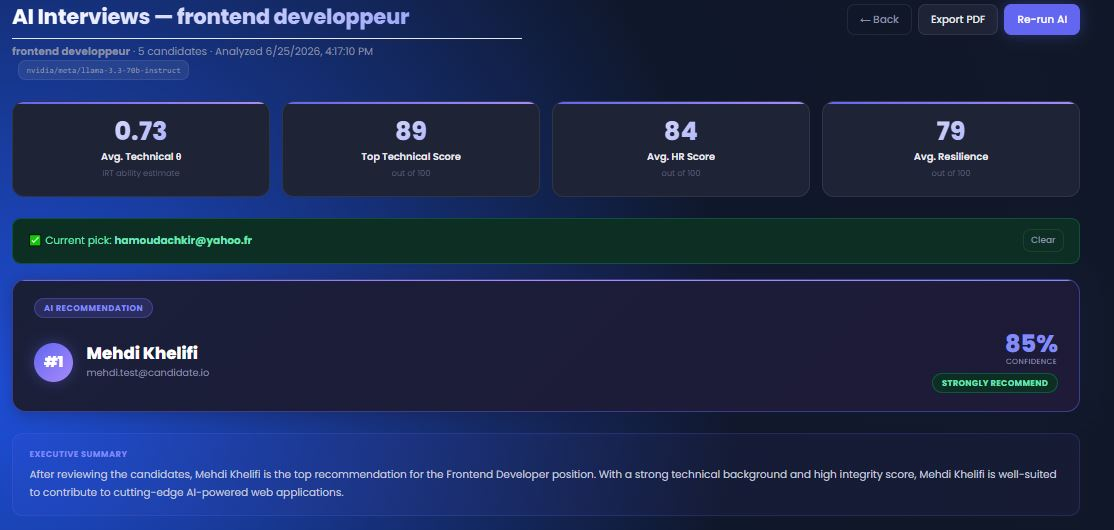
\includegraphics[width=\linewidth,keepaspectratio]{../screenshoot/compa1.JPG}
    \caption{Indicateurs agrégés et recommandation d'embauche de l'IA.}
    \label{fig:candidate-comparison-a}
  \end{subfigure}
  \par\medskip
  \begin{subfigure}{0.6\textwidth}
    \centering
    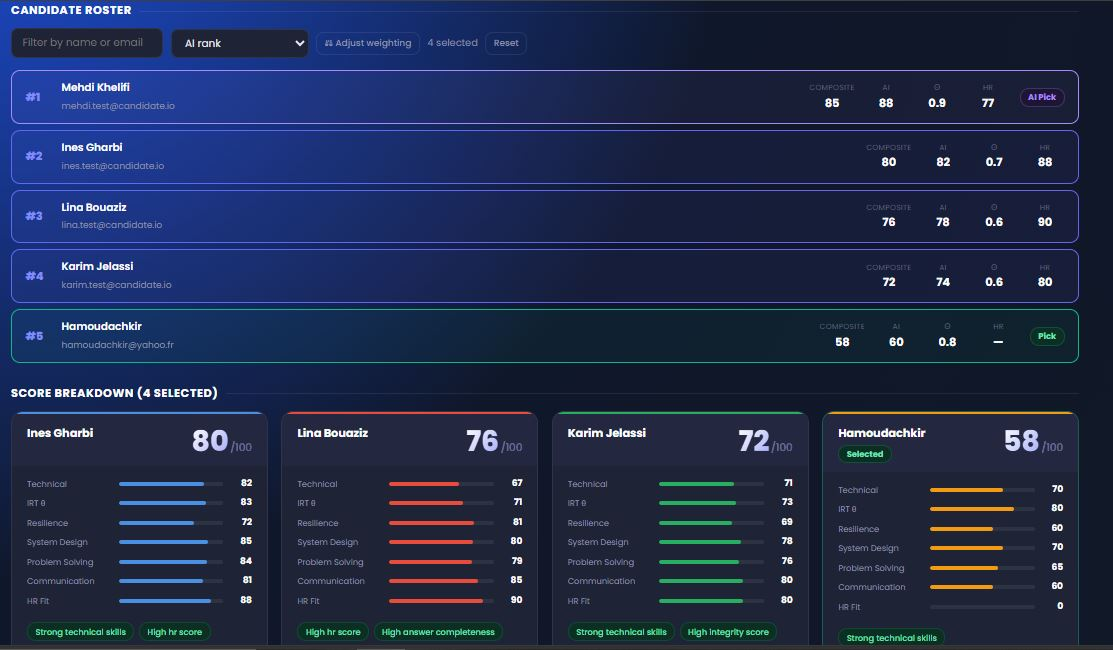
\includegraphics[width=\linewidth,keepaspectratio]{../screenshoot/compa2.JPG}
    \caption{Classement des candidats et détail des scores par dimension.}
    \label{fig:candidate-comparison-b}
  \end{subfigure}
  \par\medskip
  \begin{subfigure}{0.6\textwidth}
    \centering
    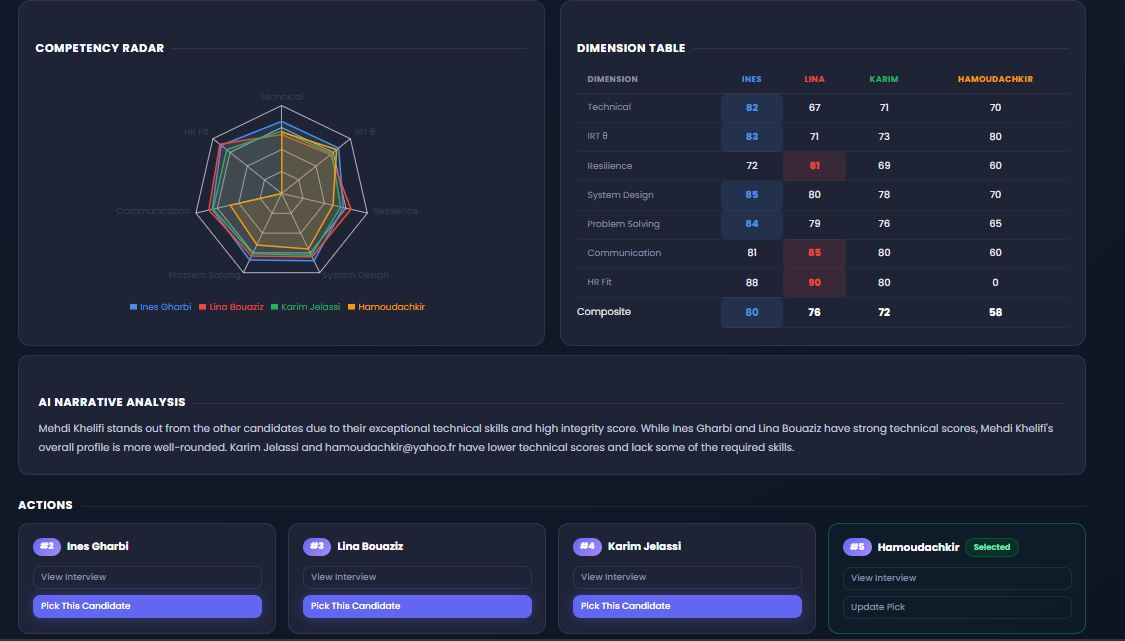
\includegraphics[width=\linewidth,keepaspectratio]{../screenshoot/compa3.JPG}
    \caption{Radar de compétences, tableau comparatif des dimensions et analyse narrative.}
    \label{fig:candidate-comparison-c}
  \end{subfigure}
  \caption{Écran de comparaison et de classement des candidats pour un poste.}
  \label{fig:candidate-comparison}
\end{figure}

\subsection{Écran de revue d'entretien}

L'écran de revue permet au recruteur d'examiner en détail un entretien terminé. Il affiche
en en-tête le nom du candidat, le poste concerné et la date de l'entretien. En dessous, une
transcription interactive liste chaque question posée par l'agent, la réponse du candidat,
le score et la justification produits par l'évaluation pondérée, ainsi que les éventuelles
violations détectées. Le rapport d'intégrité associé (niveau de risque, chronologie des
événements, recommandation) est présenté en regard, sans génération de fichier PDF externe
(figure~\ref{fig:interview-review}).

\begin{figure}[H]
  \centering
  \screenshot{interview-review.JPG}{Revue d'entretien : transcription, scores, intégrité}
  \caption{Écran de revue d'entretien côté recruteur.}
  \label{fig:interview-review}
\end{figure}

\subsection{Tableau de bord administrateur}

NextHire intègre un espace d'administration séparé, accessible sous le préfixe
\texttt{/dashboard}, protégé par un gardien de route dédié (\texttt{AdminProtectedRoute}).
Cet espace offre une vue centralisée de l'ensemble de la plateforme sans être lié à un
compte recruteur particulier.

\subsubsection{Vue d'ensemble et indicateurs clés}

La page d'accueil du tableau de bord agrège en temps réel les données de la plateforme via
l'endpoint \texttt{GET /api/admin/stats}. Six cartes d'indicateurs sont affichées en grille~:
le nombre de candidats inscrits, d'entreprises enregistrées, d'offres publiées, de
candidatures reçues, d'entretiens créés et d'entretiens planifiés. Deux graphiques complètent
cette vue~: un diagramme en anneau (\textit{donut chart}) représentant la répartition des
offres par statut, et un histogramme miniature indiquant l'évolution des candidatures dans
le temps. Un second diagramme en anneau distingue les entretiens confirmés des entretiens
en attente de planification (figure~\ref{fig:admin-dashboard}).

\begin{figure}[H]
  \centering
  \screenshot{admin-dashboard.JPG}{Tableau de bord admin : KPI, graphiques, listes récentes}
  \caption{Tableau de bord administrateur~: indicateurs en temps réel et graphiques d'activité.}
  \label{fig:admin-dashboard}
\end{figure}

\subsubsection{Gestion des entités}

La barre de navigation latérale donne accès à cinq sections de gestion~:

\begin{itemize}
  \item \textbf{Candidates} (\texttt{/dashboard/manage-candidates}) : liste paginée des
        candidats avec leurs informations de profil et leur statut de vérification.
  \item \textbf{Companies} (\texttt{/dashboard/manage-employees}) : gestion des comptes
        entreprise et de leurs informations administratives.
  \item \textbf{Jobs} (\texttt{/dashboard/jobs}) : consultation de toutes les offres publiées
        sur la plateforme, indépendamment de l'entreprise propriétaire.
  \item \textbf{Calendar} (\texttt{/dashboard/calendar}) : vue calendrier des entretiens
        planifiés sur l'ensemble des salles actives.
  \item \textbf{Settings} (\texttt{/dashboard/settings}) : paramètres globaux de la
        plateforme.
\end{itemize}

Cet espace d'administration permet de superviser l'activité de la plateforme et de
corriger d'éventuelles anomalies sans intervenir directement dans les comptes utilisateurs,
conformément au principe de séparation des responsabilités retenu lors de la conception.

\subsection{Messagerie et assistant conversationnel (NextBot)}

Au-delà du pipeline d'entretien, la page d'accueil intègre deux fonctionnalités
transverses visant à enrichir l'expérience candidat~: une messagerie directe avec le
recruteur et un assistant conversationnel alimenté par un LLM.

\subsubsection{Messagerie candidat--recruteur}

Les échanges sont persistés via un modèle \texttt{Message} (expéditeur, destinataire,
texte, horodatage, statut de lecture) exposé par une API REST dédiée
(\texttt{POST /api/messages/send}, \texttt{GET /api/messages/history/:user1/:user2},
\texttt{GET /api/messages/user/:userId}). La livraison en temps réel repose sur Socket.IO~:
l'émission d'un message déclenche un événement \texttt{send-message} côté serveur, relayé
au destinataire via \texttt{receive-message}, tandis que l'historique de la conversation est
chargé par requête REST à l'ouverture de la discussion. Le composant \texttt{MessagePopup}
fournit l'interface de discussion, réutilisée à la fois pour les échanges entre utilisateurs
et pour les interactions avec l'assistant.

\begin{figure}[H]
  \centering
  \screenshot{messaging.JPG}{Messagerie candidat--recruteur sur la page d'accueil}
  \caption{Interface de messagerie candidat--recruteur.}
  \label{fig:messaging}
\end{figure}

\subsubsection{NextBot : assistant conversationnel}

Le chatbot, nommé NextBot, est traité comme un utilisateur spécial (identifiant
\texttt{"bot"}) au sein de la même infrastructure de messagerie plutôt que comme un service
indépendant. Les requêtes adressées au bot (\texttt{POST /api/messages/bot/interaction})
sont transmises à l'API Groq (compatible OpenAI), via le modèle \texttt{gpt-oss-120b}. Pour
contextualiser ses réponses, le service enrichit le \textit{prompt} système avec le profil du
candidat (compétences, expérience) ainsi que les six derniers échanges de la conversation,
ce qui lui permet de fournir des conseils personnalisés sur la recherche d'emploi, la
préparation aux entretiens et la navigation sur la plateforme, sans recourir à une base
vectorielle~: il s'agit d'un enrichissement de contexte directement puisé dans MongoDB,
et non d'une recherche par similarité.

\begin{figure}[H]
  \centering
  \screenshot{chatbot.JPG}{Assistant conversationnel NextBot sur la page d'accueil}
  \caption{Assistant conversationnel NextBot.}
  \label{fig:chatbot}
\end{figure}

\section{Sécurité et conformité}

La sécurité de NextHire repose sur une stratégie de défense en profondeur : plusieurs couches
indépendantes couvrent l'identité, l'autorisation, la protection contre les abus, l'intégrité
de l'entretien et la conformité réglementaire. Cette section consolide l'ensemble des mécanismes
implémentés dans la plateforme.

\subsection{Autorisation par rôles -- RBAC}

Le contrôle d'accès basé sur les rôles est assuré par le middleware \texttt{requireEnterprise},
appliqué à tous les points de terminaison réservés aux recruteurs. Son comportement suit deux
chemins :

\begin{itemize}
  \item \textbf{Chemin rapide.} Si le JWT porte le champ \texttt{role = 'ENTERPRISE'},
        l'accès est accordé immédiatement sans requête base de données.
  \item \textbf{Repli base de données.} Pour les jetons antérieurs ne portant pas encore
        le champ \texttt{role} (compatibilité ascendante), le middleware interroge MongoDB
        (\texttt{User.findById().select('role').lean()}) et met à jour \texttt{req.user.role}
        en mémoire pour les middlewares aval.
\end{itemize}

Toute requête dont le rôle ne correspond pas à \texttt{ENTERPRISE} reçoit une réponse
\texttt{HTTP 403} avant d'atteindre la logique métier. Cette approche \textit{fail-closed}
garantit qu'une erreur de configuration (jeton sans rôle, base indisponible) bloque l'accès
plutôt que de l'autoriser par défaut.

\subsection{Limitation de débit}

Deux limiteurs de débit indépendants, fondés sur \texttt{express-rate-limit}, protègent les
points de terminaison à risque élevé, comme le récapitule le tableau~\ref{tab:rate-limiters}.

\begin{table}[H]
  \centering
  \footnotesize
  \renewcommand{\arraystretch}{1.3}
  \begin{tabularx}{\textwidth}{|>{\raggedright\arraybackslash}p{3.5cm}|>{\raggedright\arraybackslash}X|>{\raggedright\arraybackslash}p{2.8cm}|}
    \hline
    \textbf{Limiteur} & \textbf{Règle} & \textbf{Clé de comptage} \\
    \hline
    \texttt{aiGenerationRateLimiter} & 10 requêtes par minute par utilisateur (configurable via \texttt{AI\_GENERATION\_MAX\_PER\_MINUTE}) & \texttt{req.user.\_id} (repli sur IP) \\
    \hline
    \texttt{quizRateLimiter} & 3 soumissions par tranche de 24\,h par couple candidat\,+\,offre (configurable via \texttt{QUIZ\_MAX\_ATTEMPTS\_PER\_DAY}) & \texttt{candidateId-jobId} (repli sur IP) \\
    \hline
  \end{tabularx}
  \caption{Limiteurs de débit de la plateforme NextHire.}
  \label{tab:rate-limiters}
\end{table}

Les deux limiteurs partagent la même architecture de stockage : en développement, un compteur
en mémoire est utilisé ; en production, un stockage Redis (\texttt{rate-limit-redis}) est activé
par la variable d'environnement \texttt{QUIZ\_RATE\_LIMIT\_USE\_REDIS=true}. En cas d'échec de
connexion à Redis, le système se replie automatiquement sur le compteur en mémoire avec un
avertissement journalisé. Les requêtes ayant échoué à la validation (\textit{skipFailedRequests})
ne sont pas décomptées du quota.

\subsection{Conformité RGPD}

La plateforme a été conçue pour respecter les principes du Règlement Général sur la Protection
des Données :

\begin{itemize}
  \item \textbf{Consentement explicite.} Le candidat est informé, lors de l'enrôlement facial
        et avant le démarrage de l'entretien, que sa webcam et son microphone sont activés
        à des fins d'évaluation. L'entretien ne peut commencer sans validation de cette étape.
  \item \textbf{Minimisation des données biométriques.} Les trames webcam transmises au
        serveur pour la vérification faciale et la détection d'objets sont traitées en
        mémoire et ne sont jamais persistées~; seuls les embeddings (vecteurs de
        512 dimensions) qui en résultent sont conservés.
  \item \textbf{Décision finale humaine.} Le rapport post-entretien généré par l'IA fournit
        des scores, des points forts et des lacunes, et se conclut par une recommandation
        (\textit{Strong Hire / Hire / Maybe / No Hire}) ; la décision finale
        d'acceptation ou de refus reste une action explicite du recruteur, tracée en base de
        données. L'IA n'embauche pas : elle informe.
  \item \textbf{Chiffrement des données en transit.} Toutes les communications entre le
        navigateur et les services backend sont protégées par TLS (HTTPS). Les mots de
        passe ne sont jamais stockés en clair : seul leur condensé (\texttt{bcrypt} ou
        \texttt{bcryptjs} selon le module) est persisté.
\end{itemize}

\section{Tests et validation}

\subsection{Stratégie de tests et outillage}

La validation de NextHire suit le principe de la pyramide des tests : une base large de tests
unitaires rapides et isolés, un étage intermédiaire de tests d'intégration qui éprouvent les
frontières entre composants, et un sommet plus étroit de tests de bout en bout et de validation
système. Les dépendances lourdes (modèles PyTorch, Faster-Whisper, YOLO, accès réseau aux
API Groq et Edge TTS, MongoDB, Redis) sont remplacées par des doublures
(\textit{stubs} enregistrés dans \texttt{sys.modules} côté Python, données factices côté
Node.js), de sorte que la suite s'exécute en quelques secondes, sans GPU ni clé d'API. Les
tests qui exigent une infrastructure réelle sont isolés et ignorés automatiquement lorsque
celle-ci est absente. Le tableau~\ref{tab:test-frameworks} récapitule les frameworks employés
par service et par niveau.

\begin{table}[H]
  \centering
  \footnotesize
  \renewcommand{\arraystretch}{1.3}
  \setlength{\tabcolsep}{5pt}
  \begin{tabularx}{\textwidth}{|>{\raggedright\arraybackslash}p{3.4cm}|>{\raggedright\arraybackslash}p{2.3cm}|>{\raggedright\arraybackslash}p{3.0cm}|>{\raggedright\arraybackslash}X|}
    \hline
    \rowcolor{blue!10}
    \textbf{Service} & \textbf{Niveau} & \textbf{Framework} & \textbf{Fichier représentatif} \\
    \hline
    Backend Node.js & Unitaire & \texttt{node:assert} & \texttt{faceVerifyDecision.test.js} \\
    \hline
    Moteur d'entretien (\texttt{voice\_engine}) & Unitaire & \texttt{unittest} + stubs & \texttt{test\_interview\_agent\_conversation.py} \\
    \hline
    Service d'analyse (\texttt{analysis\_service}) & Unitaire / intégration & \texttt{pytest} & \texttt{test\_report\_schema.py} \\
    \hline
    Frontend (React) & Bout en bout & Playwright & \texttt{e2e-rh-job-match.spec.js} \\
    \hline
    Système & Validation & Scripts Python & \texttt{tests/} (charge, chaos, ML, intégrité) \\
    \hline
  \end{tabularx}
  \caption{Frameworks de test par service et par niveau.}
  \label{tab:test-frameworks}
\end{table}

\subsection{Tests unitaires du service d'analyse}

Le service d'analyse post-entretien constitue la suite la plus fournie : neuf modules de tests
\texttt{pytest} sous \texttt{analysis\_service/tests/}. Ils couvrent la validation du schéma de
rapport (\texttt{report\_schema}), la fusion et le polissage des rapports, l'extraction des
métadonnées d'entretien, le service FFmpeg et le service média. Le tableau~\ref{tab:analysis-tests}
détaille la répartition et les résultats d'exécution.

\begin{table}[H]
  \centering
  \footnotesize
  \renewcommand{\arraystretch}{1.25}
  \setlength{\tabcolsep}{6pt}
  \begin{tabularx}{\textwidth}{|>{\raggedright\arraybackslash}X|>{\centering\arraybackslash}p{2.0cm}|>{\centering\arraybackslash}p{2.0cm}|}
    \hline
    \rowcolor{blue!10}
    \textbf{Module de test} & \textbf{Tests} & \textbf{Réussis} \\
    \hline
    \texttt{test\_enhanced\_report.py} & 48 & 48 \\ \hline
    \texttt{test\_media\_service.py} & 33 & 33 \\ \hline
    \texttt{test\_report\_polish\_merge.py} & 22 & 22 \\ \hline
    \texttt{test\_ffmpeg\_service.py} & 19 & 19 \\ \hline
    \texttt{test\_interview\_metadata.py} & 19 & 19 \\ \hline
    \texttt{test\_phase2\_features.py} & 18 & 17 (1 ignoré) \\ \hline
    \texttt{test\_report\_schema.py} & 15 & 15 \\ \hline
    \texttt{test\_report\_quality.py} & 9 & 9 \\ \hline
    \texttt{test\_report\_new\_fields.py} & 8 & 8 \\ \hline
    \rowcolor{gray!8}
    \textbf{Total} & \textbf{191} & \textbf{190 (1 ignoré)} \\ \hline
  \end{tabularx}
  \caption{Résultats d'exécution des tests unitaires du service d'analyse.}
  \label{tab:analysis-tests}
\end{table}

\subsection{Tests d'intégration, de bout en bout et de validation système}

\paragraph{Bout en bout (Frontend).} Un scénario Playwright
(\texttt{e2e-rh-job-match.spec.js}) pilote un navigateur réel pour valider le parcours
recruteur d'appariement candidat~/~offre (\textit{job match}) à travers l'application et le
backend. Ce test nécessite la pile complète en cours d'exécution et est donc exécuté lors des
campagnes d'intégration.

\paragraph{Validation système (suite Phase~6).} Le répertoire \texttt{tests/} à la racine
regroupe une suite de validation système couvrant plusieurs préoccupations transversales :
tests de charge (\texttt{load/} : \textit{locust}, exécution concurrente d'entretiens, charge
WebSocket), tests de robustesse (\texttt{chaos/} : pannes simulées de MongoDB, de Redis, du
\textit{worker} et expiration GPU), validation ML (\texttt{ml/} : détection de dérive et
validation en mode ombre), intégrité des rapports (\texttt{integrity/}) et audit de cohérence
(\texttt{audit/} : détection d'orphelins, rejeu déterministe). Ces tests s'exécutent contre une
infrastructure vivante et sont déclenchés manuellement lors des campagnes de validation.

\subsection{Synthèse cumulative}

Le tableau~\ref{tab:cumulative-tests} consolide le décompte et les taux de réussite des tests
automatisés exécutés sans infrastructure externe. L'ensemble des 199~tests unitaires
(\texttt{pytest} et \texttt{unittest}) ainsi que les 12~assertions du test Node.js réussissent,
soit un taux de réussite de 100~\%. Chaque dépendance native lourde est interceptée avant import,
ce qui permet à la suite de s'exécuter en quelques secondes.

\begin{table}[H]
  \centering
  \footnotesize
  \renewcommand{\arraystretch}{1.25}
  \setlength{\tabcolsep}{6pt}
  \begin{tabularx}{\textwidth}{|>{\raggedright\arraybackslash}X|>{\centering\arraybackslash}p{1.8cm}|>{\centering\arraybackslash}p{1.8cm}|>{\centering\arraybackslash}p{2.0cm}|}
    \hline
    \rowcolor{blue!10}
    \textbf{Service} & \textbf{Fichiers} & \textbf{Tests} & \textbf{Taux de réussite} \\
    \hline
    \texttt{analysis\_service} (pytest) & 9 & 190 & 100~\% \\ \hline
    \texttt{voice\_engine} (unittest) & 2 & 9 & 100~\% \\ \hline
    Backend Node.js (\texttt{node:assert}) & 1 & 12 assertions & 100~\% \\ \hline
    Frontend (Playwright, E2E) & 1 & 2 scénarios & infrastructure requise \\ \hline
    \rowcolor{gray!8}
    \textbf{Total (hors infrastructure)} & \textbf{12} & \textbf{211 vérifications} & \textbf{100~\%} \\ \hline
  \end{tabularx}
  \caption{Synthèse cumulative des tests automatisés de NextHire.}
  \label{tab:cumulative-tests}
\end{table}

\subsection{Couverture de code}

La couverture du service d'analyse a été mesurée avec \texttt{pytest-cov}. Sur l'ensemble du
paquet \texttt{app} (4218~instructions), la suite couvre 45~\% des instructions. Cette valeur
globale reflète un choix de périmètre délibéré : les tests ciblent en priorité le cœur métier
(schéma et construction des rapports, évaluation des questions, appariement aux offres,
services média), tandis que les couches d'infrastructure (workers RQ, registre de modèles ML
multi-locataires, RBAC, métriques) sont éprouvées au niveau de l'intégration système. Le
tableau~\ref{tab:analysis-coverage} présente la couverture des modules les plus exercés.

\begin{table}[H]
  \centering
  \footnotesize
  \renewcommand{\arraystretch}{1.25}
  \setlength{\tabcolsep}{6pt}
  \begin{tabularx}{\textwidth}{|>{\raggedright\arraybackslash}X|>{\centering\arraybackslash}p{2.6cm}|}
    \hline
    \rowcolor{blue!10}
    \textbf{Module} & \textbf{Couverture (instructions)} \\
    \hline
    \texttt{schemas/report\_schema.py} & 99~\% \\ \hline
    \texttt{services/report\_service.py} & 91~\% \\ \hline
    \texttt{services/question\_evaluator.py} & 89~\% \\ \hline
    \texttt{services/sentiment\_service.py} & 86~\% \\ \hline
    \texttt{services/job\_match\_service.py} & 84~\% \\ \hline
    \texttt{services/ffmpeg\_service.py} & 81~\% \\ \hline
    \texttt{services/qna\_service.py} & 79~\% \\ \hline
    \texttt{services/interview\_metadata.py} & 54~\% \\ \hline
    \rowcolor{gray!8}
    \textbf{Ensemble du paquet \texttt{app}} & \textbf{45~\%} \\ \hline
  \end{tabularx}
  \caption{Couverture d'instructions par module du service d'analyse (\texttt{pytest-cov}).}
  \label{tab:analysis-coverage}
\end{table}

\section{Conclusion}

Ce dernier sprint a complété NextHire par ses fonctionnalités d'aide à la décision, analyse multimodale, comparaison et classement des candidats, revue d'entretien, et par son tableau de bord administrateur, tout en renforçant la sécurité et la conformité RGPD. La suite de tests automatisés (211~vérifications, taux de réussite de 100~\% hors infrastructure) et les mesures de performance valident la faisabilité technique de la solution. La conclusion générale du rapport reviendra sur les apports de la plateforme et ses perspectives d'évolution.
